\section{Question 3}
     \hspace*{0.6cm}\textbf{Hãy project hình vào hình chữ nhật di chuyển trong movie sau}
     \begin{figure}[H]
          \centering
          
\includegraphics[width=0.6\textwidth]{pictures/section3/s3_p02_picture.png}
          \caption{Hình ảnh cần project}
          \label{s3_p02_picture}
     \end{figure}
     \begin{figure}[H]
          \centering
          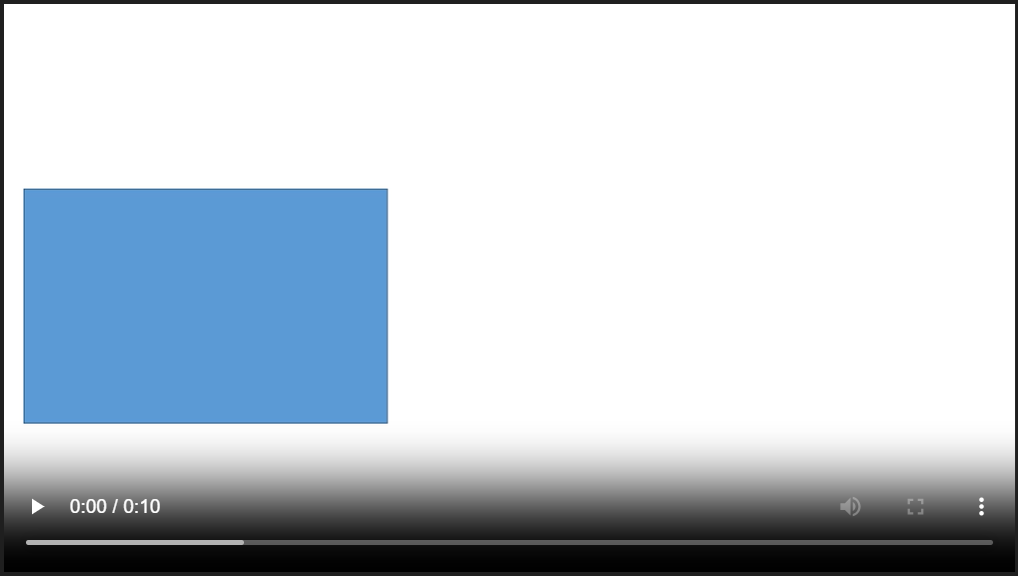
\includegraphics[width=0.6\textwidth]{pictures/section3/s3_p01_movie.png}
          \caption{Movie}
          \label{s3_p01_movie}
     \end{figure}
     \subsection{Ý tưởng}
          \hspace*{0.6cm}Tìm 4 điểm tương ứng giữa hình chữ nhật xanh trong movie ở từng frame, sau đó sử dụng hàm \texttt{cv2.findHomography} để lấy ma trận biến đổi phối cảnh và sau đó sử dụng hàm \texttt{cv2.warpPerspective} để thực hiện phép biến đổi, cuối cùng ghép hình đã biến đổi vào vị trí hình chữ nhật xanh trong movie.
     \subsection{Các bước thực hiện}
          \begin{itemize}
               \item \textbf{Bước 1: Đọc video và hình ảnh cần project.}
               \begin{itemize}[label={--}]
                    \item Chương trình chạy hàm đọc hình ảnh, video cùng với các thông số của video và hình ảnh như FPS, chiều rộng, chiều cao, tổng số frame của video.
                    \begin{lstlisting}
# Step 1: Load video and image resources
def load_resources(video_path, image_path):
    source_image = cv2.imread(image_path)
    if source_image is None:
        raise ValueError("Cannot read source image!")

    cap = cv2.VideoCapture(video_path)
    if not cap.isOpened():
        raise ValueError("Cannot open video!")
    fps = int(cap.get(cv2.CAP_PROP_FPS))
    width = int(cap.get(cv2.CAP_PROP_FRAME_WIDTH))
    height = int(cap.get(cv2.CAP_PROP_FRAME_HEIGHT))
    total_frames = int(cap.get(cv2.CAP_PROP_FRAME_COUNT))

    h, w = source_image.shape[:2]
    source_is_horizontal = w > h

    print(f"Video info: {width}x{height} @ {fps}fps, {total_frames} frames")
    print(f"Source image: {w}x{h}, Orientation: {'Horizontal' if source_is_horizontal else 'Vertical'}")

    return cap, source_image, fps, width, height, total_frames, source_is_horizontal
                    \end{lstlisting}
               \end{itemize}
               \item \textbf{Bước 2: Detect hình chữ nhật xanh trong từng frame của video.}
               \begin{itemize}[label={--}]
                    \item Chuyển hình ảnh về không gian màu HSV.
                    \item Tạo 1 mask để lọc ra vùng màu xanh với các ngưỡng được tinh chỉnh như sau, kết quả thu được là ảnh nhị phân
                    \begin{lstlisting}[language=Python]
lower_blue = np.array([90, 100, 100])
upper_blue = np.array([130, 255, 255])
mask = cv2.inRange(hsv, lower_blue, upper_blue)
                    \end{lstlisting}
                    \item Sau đó thực hiện các bước xử lý hình thái học rồi tìm contours, sau đó lấy contours lớn nhất là khung hình chữ nhật xanh cần project ảnh vào.
                    \begin{lstlisting}[language=Python]
kernel = np.ones((5, 5), np.uint8)
mask = cv2.morphologyEx(mask, cv2.MORPH_CLOSE, kernel)
mask = cv2.morphologyEx(mask, cv2.MORPH_OPEN, kernel)
contours, _ = cv2.findContours(mask, cv2.RETR_EXTERNAL, cv2.CHAIN_APPROX_SIMPLE)
largest_contour = max(contours, key=cv2.contourArea)
                    \end{lstlisting}
                    \item Sử dụng hàm \texttt{cv2.approxPolyDP} để lấy 4 điểm góc của hình chữ nhật.
                    \begin{lstlisting}[language=Python]
epsilon = 0.02 * cv2.arcLength(largest_contour, True)
approx = cv2.approxPolyDP(largest_contour, epsilon, True)
if len(approx) != 4:
     rect = cv2.minAreaRect(largest_contour)
     box = cv2.boxPoints(rect)
     approx = np.int0(box)
                    \end{lstlisting}     
               \end{itemize}
               \item \textbf{Bước 3: Sắp xếp 4 điểm góc theo thứ tự: trên trái, trên phải, dưới phải, dưới trái.}
               \newline
               \hspace*{0.6cm}Bước này giúp ta xác định đúng vị trí các điểm góc theo thứ tự được kí hiệu là TL (top left), TR (top right), BR (bottom right), BL (bottom left) để việc tính toán ma trận biến đổi thuận tiện.
               \begin{lstlisting}[language=Python]
# Step 3: Order points of 4 corners (TL, TR, BR, BL - clockwise)
def order_points(pts):
    rect = np.zeros((4, 2), dtype="float32")
    s = pts.sum(axis=1)
    rect[0] = pts[np.argmin(s)]  # TL
    rect[2] = pts[np.argmax(s)]  # BR

    diff = np.diff(pts, axis=1)
    rect[1] = pts[np.argmin(diff)]  # TR
    rect[3] = pts[np.argmax(diff)]  # BL

    return rect
               \end{lstlisting}
               \hspace*{0.6cm}Thuật toán xác định vị trí các điểm góc của hình chữ nhật dựa trên tổng và hiệu của tọa độ pixel x, y của các điểm nằm trên contours. Cụ thể:
               \begin{itemize}[label={--}]
                    \item Điểm có tổng tọa độ ($x + y$) nhỏ nhất được xác định là góc trên bên trái (TL)
                    \item Điểm có tổng tọa độ ($x + y$) lớn nhất được xác định là góc dưới bên phải (BR)
                    \item Điểm có hiệu tọa độ ($y - x$) nhỏ nhất được xác định là góc trên bên phải (TR)
                    \item Điểm có hiệu tọa độ ($y - x$) lớn nhất được xác định là góc dưới bên trái (BL)
               \end{itemize}
               \hspace*{0.6cm}Bước sắp xếp 4 điểm góc theo thứ tự này được thực hiện chỉ với frame đầu tiên, khi nhận xét trong video thấy rằng hình chữ nhật ban đầu nằm ngang, vậy nên thuật toán sẽ không bị nhầm lẫn trong việc xác định vị trí các điểm góc. 
               \item \textbf{Bước 4: Viết hàm để detect đúng các điểm 4 góc của hình chữ nhật trong các frame tiếp theo đúng theo thứ tự các điểm góc đã xác định ở frame trước đó.}
               \newline
               \hspace*{0.6cm}Bước này mục đích tránh việc ở các frame sau, hình chữ nhật bị xoay, và việc chỉ dùng hàm \texttt{order\_points} khiến cho thứ tự các điểm góc bị thay đổi, dẫn đến việc tính toán ma trận biến đổi làm cho hình có thể bị lật. Hàm dựa trên ý tưởng video gồm các frame ảnh tĩnh liên tiếp nhau, nên vị trí các điểm góc của hình chữ nhật trong frame hiện tại sẽ không thay đổi quá nhiều so với frame trước đó. Do đó, ta có thể so sánh khoảng cách giữa các điểm góc trong frame hiện tại với các điểm góc đã được xác định trong frame trước đó, từ đó tìm ra điểm góc tương ứng gần nhất.
               \begin{lstlisting}[language=Python]
# Step 4: Match corners with previous frame
def match_corners_with_previous(current, prev):
    matched = np.zeros_like(prev)
    used = [False] * 4

    for i in range(4):
        min_dist = float("inf")
        min_idx = -1
        for j in range(4):
            if used[j]:
                continue
            dist = np.linalg.norm(prev[i] - current[j])
            if dist < min_dist:
                min_dist = dist
                min_idx = j
        
        matched[i] = current[min_idx]
        used[min_idx] = True

    return matched
               \end{lstlisting}  
               \item \textbf{Bước 5: Tính ma trận biến đổi phối cảnh và thực hiện biến đổi.}    
               \begin{itemize}
                    \item Sử dụng hàm \texttt{cv2.findHomography} để tính ma trận biến đổi phối cảnh từ 4 điểm góc của hình ảnh cần project sang 4 điểm góc của hình chữ nhật xanh trong frame hiện tại.
               \begin{lstlisting}[language=Python]
M = cv2.findHomography(src_points, dst_points)[0]
               \end{lstlisting}
               \item Với \texttt{src\_points} là 4 điểm góc của hình cần project, cũng được sắp xếp theo thứ tự TL, TR, BR, BL.
               \begin{lstlisting}[language=Python]
h, w = source_image.shape[:2]

src_points = np.array([
     [0, 0],          # TL
     [w - 1, 0],      # TR
     [w - 1, h - 1],  # BR
     [0, h - 1]       # BL
], dtype="float32")
               \end{lstlisting}    
               \item Sau đó sử dụng hàm \texttt{cv2.warpPerspective} để thực hiện phép biến đổi 
               \begin{lstlisting}[language=Python]
warped = cv2.warpPerspective(source_image, M, (frame.shape[1], frame.shape[0]))
               \end{lstlisting}   
               \item Cuối cùng ghép hình đã biến đổi vào vị trí hình chữ nhật xanh trong frame.              
               \begin{lstlisting}[language=Python]
mask = np.zeros((frame.shape[0], frame.shape[1]), np.uint8)
cv2.fillConvexPoly(mask, np.int32(corners), 255)
mask3 = cv2.cvtColor(mask, cv2.COLOR_GRAY2BGR)

bg = cv2.bitwise_and(frame, cv2.bitwise_not(mask3))
fg = cv2.bitwise_and(warped, mask3)

return cv2.add(bg, fg)
               \end{lstlisting}               
               \end{itemize}  
               \item  \textbf{Kết quả:} Hình ảnh sau khi được warp và ghép, ở những frame mà hình chữ nhật xoay, hình ảnh cũng xoay theo đúng hướng của hình chữ nhật, không bị lật ngược.   
               \begin{figure}[H]
                    \centering
                    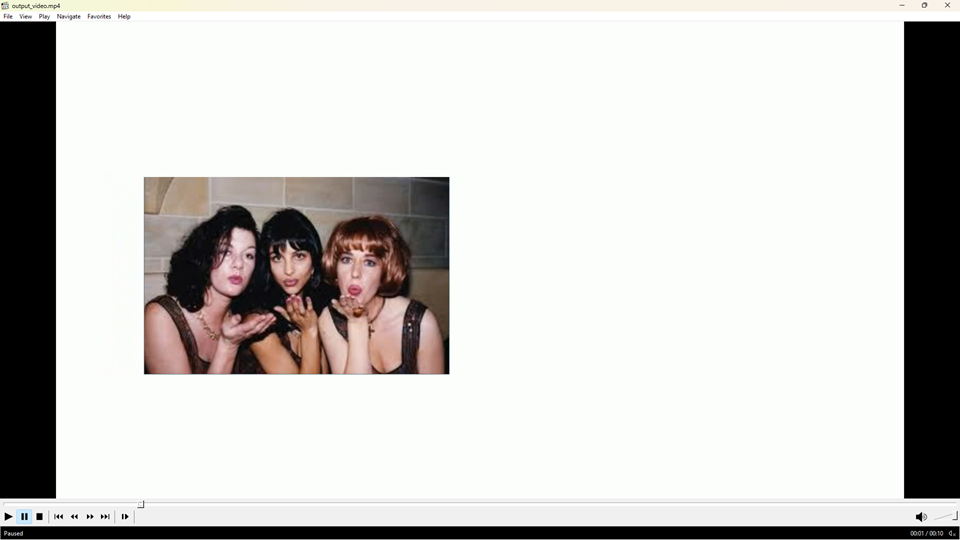
\includegraphics[width=0.6\textwidth]{pictures/section3/s3_p03_result_01.png}
                    \label{s3_p03_result}
               \end{figure}
               \begin{figure}[H]
                    \centering
                    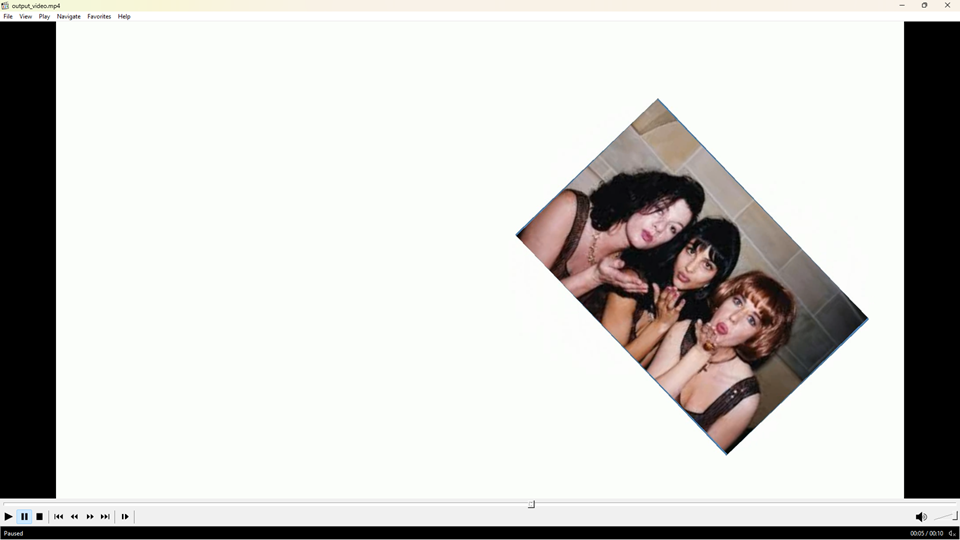
\includegraphics[width=0.6\textwidth]{pictures/section3/s3_p04_result_02.png}
                    \label{s3_p04_result}
               \end{figure}
               \begin{figure}[H]
                    \centering
                    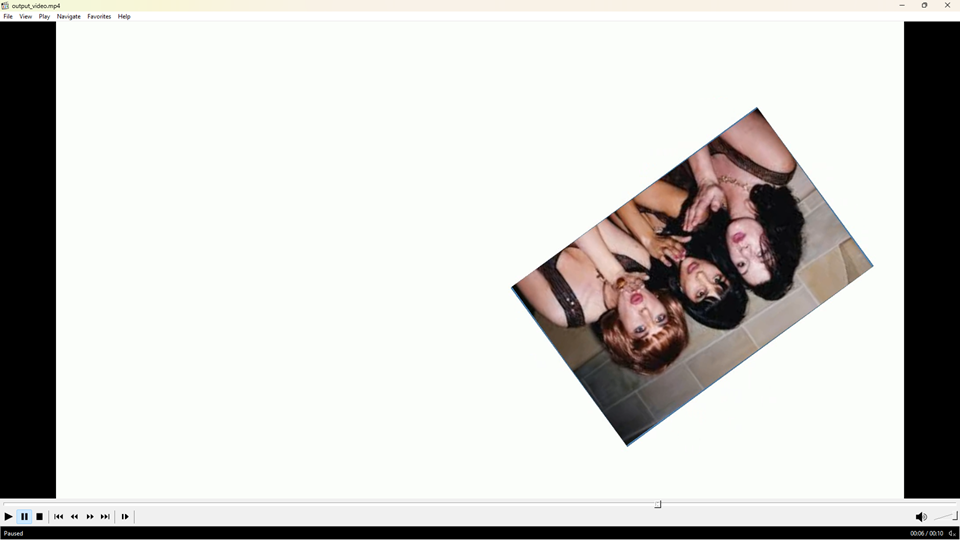
\includegraphics[width=0.6\textwidth]{pictures/section3/s3_p05_result_03.png}
                    \label{s3_p05_result}
               \end{figure}
          \end{itemize}
